% 20 Apr 2014 : GWA : 0.5 pages

\section{Implementation}
\label{sec-implementation}

\begin{figure}[t]

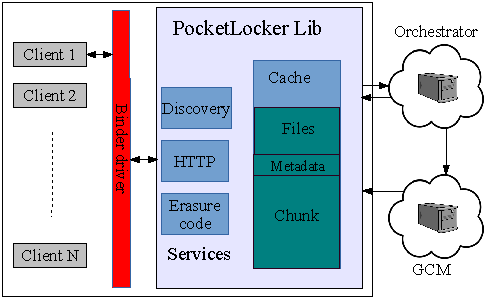
\includegraphics[width=0.9\columnwidth]{./figures/implementation.pdf}

\caption{\small \textbf{Architecture.} The figure illustrates the different
  components in the implementation of PocketLocker.}

\label{fig-implementation}
  \vspace*{-0.2in}

\end{figure}

We have implemented PocketLocker PSC as an Android background service on both
interactive and fixed non-interactive devices. Galaxy Nexus and Nexus 5
smartphones constituted the mobile interactive devices, and Android x86
virtual machines~\cite{androidx86} running on desktops served as the fixed
non-interactive. The PocketLocker service runs in the background and exposes
APIs to provide clients access to the files stored in the user's PSC. It also
maintains chunk placement in the cache as directed by the orchestrator. 

We chose to implement PocketLocker as a user application rather than
integrating the service with the file system so that users do not need root
privileges to install PocketLocker on their devices and PocketLocker can be
distributed via the Android Play Store.~\cite{playstore} On both interactive
and non-interactive devices, the PocketLocker service maintains the local file
and chunk cache according to the placement directions calculated by the
orchestrator. On fixed devices, PocketLocker also offers two network services.
The discovery service responds to chunk requests that are issued by interactive
devices on the same local network. The HTTP service facilitates the transfer of
newly created files and chunks among the user's PSC devices as per the chunk
placement scheme.

PocketLocker exposes its APIs both to the orchestrator, to receive local cache
maintenance directions, and to local client applications, to provide access to
user files. PocketLocker clients interact with the PocketLocker service via the
\textit{binder} driver framework in Android. The binder facilitates thread safe
inter process communication in Android. The orchestrator was implemented using
the Tornado and Flask web frameworks. The orchestrator listens to status
updates by the user's PSC devices and tracks and maintains the cache
information at each of the devices in the user's PSC using an \textit{SQLite}
database. To push information to user's PSC device, the orchestrator uses the
Google Cloud Messaging (GCM) framework to communicate information about new
file creation and chunk placement with the user's PocketLocker devices.
